\documentclass[[a4paper,11pt]{article}
\renewcommand{\rmdefault}{ptm}
\usepackage[scaled=0.92]{helvet}
\usepackage{courier,xcolor,colortbl,listings,parskip,graphicx,fancyvrb,fancyhdr,lastpage}
\usepackage{float,framed}
\usepackage{epigraph}
\epigraphsize{\small\itshape}
\setlength\epigraphwidth{8cm}
\setlength\epigraphrule{0pt}
\normalfont
\usepackage[T1]{fontenc}
\setlength{\parskip}{7pt}
\usepackage[toc,page]{appendix}
\usepackage[hmargin=2.5cm,vmargin=2cm]{geometry}
\usepackage[utf8]{inputenc}
\usepackage[brazil]{babel}
\pagestyle{fancy}
\setlength{\headheight}{120pt}
\setlength{\headsep}{30pt}
\setlength{\textheight}{550pt}
\renewcommand{\headrulewidth}{0pt}
\lhead{}
\rhead{}
\chead{
\includegraphics{brasao.jpg}\\
        \large \textbf{PRESIDÊNCIA DA REPÚBLICA}\\
        \large SECRETARIA-GERAL\\
        \large Secretaria-Executiva}
\cfoot{}
\rfoot{\thepage /\pageref{LastPage}}
\hyphenation{par-ti-ci-pa-ção}
\hyphenation{ad-mi-nis-tra-dor}
\bibliographystyle{ieeetr}

\newcommand{\MyName}{Daniela Soares Feitosa}
\newcommand{\MyEmail}{daniela@colivre.coop.br}
\newcommand{\ContractNumber}{2013/000292}
\newcommand{\ProjectCode}{Projeto PNUD BRA/12/018}
\newcommand{\NomeSecretaria}{Secretaria Geral da Presidência da República}
\newcommand{\SiglaSecretaria}{SG/PR}
\newcommand{\ProductNumber}{01}
\newcommand{\ProductDescription}{Documento técnico com complementação da 
documentação de instalação e uso da plataforma Noosfero contendo
conceitos e tutoriais.}
\newcommand{\MesEntrega}{Setembro de 2013}
\newcommand{\DiaEntrega}{23}

\begin{document}
\lstset{language=Ruby}
\definecolor{light-gray}{gray}{0.95}
\lstdefinestyle{codeFrame}{backgroundcolor=\color{light-gray},frame=lines}

\textbf{\ProjectCode \ -} \ProductDescription

\vspace{3cm}

\begin{minipage}{0.5\textwidth}
  \textbf{Consultora: \MyName}
  \newline
  \textbf{Contrato nº: \ContractNumber}
  \newline
  \textbf{Produto / nº: \ProductNumber}
\end{minipage}

\vspace{2cm}

\textbf{Assinatura do Consultor}

\begin{framed}
Local e data: Brasília/DF, \line(1,0){20} \ de \line(1,0){100} \ de 2014
\newline
\newline
Assinatura do Consultor: \line(1,0){300}
\end{framed}

\vspace{1cm}

\textbf{Assinatura do Supervisor}

\begin{framed}
Atesto que os serviços foram prestados conforme estabelecido no Contrato
de Consultoria.
\newline
\newline
Local e data: Brasília/DF, \line(1,0){20} \ de \line(1,0){100} \ de 2014
\newline
\newline
Assinatura e Carimbo: \line(1,0){300}
\end{framed}

\clearpage
\newcolumntype{g}{>{\columncolor{light-gray}}l}

\begin{center}
  \begin{tabular}{| g | p{10cm} |}
    \hline
    \textbf{Título} & \ProductDescription \\ \hline
    \textbf{Língua do documento} & Português - Brasil \\ \hline
    \textbf{Documentação de referência} & Português \\ \hline
    \textbf{Unidade responsável} & \NomeSecretaria \
(\SiglaSecretaria) \\ \hline
    \textbf{Criador} & \MyName - \MyEmail \\ \hline
    \textbf{Taxonomias} & Desenvolvimento \\ \hline
    \textbf{Data de aprovação} &  \\ \hline
    \textbf{Público} & \SiglaSecretaria, Parceiros e Sociedade
Civil \\ \hline
    \textbf{Faz parte do} & \ProjectCode \\ \hline
    \textbf{Em conformidade com a} & \NomeSecretaria \\ \hline
    \textbf{Documentos anexos} & Página da Comunidade OSC - Organizações da
Sociedade Civil; CSS do cabeçalho do tema de comunidade; Código javascript para
incluir uma classe identificadora; Código CSS para estilizar os blocos com o padrão
colorido \\ \hline
    \textbf{Revisado em} &  \\ \hline
  \end{tabular}
\end{center}

\clearpage

\tableofcontents
\clearpage
\listoffigures

\clearpage

\section{Apresentação}

Em consonância com os objetivos e cronograma previsto no âmbito do
projeto BRA/12/018:
\textbf{Desenvolvimento de Metodologias de Articulação e Gestão de
Políticas Públicas para Promoção da Democracia Participativa},
firmado entre a Secretaria-Geral da Presidência da República
(SG/PR) e o Programa das Nações Unidas para o Desenvolvimento (PNUD),
o presente documento apresenta o documento técnico com complementação da 
documentação de instalação e uso da plataforma Noosfero contendo
conceitos e tutoriais. 

Esse documento está configurado como produto 1 da consultoria técnica
para especificação da construção dos códigos das metodologias de
organização da informação e interação participativa do portal de
participação social.

Neste documento serão apresentados os conceitos que envolvem a
plataforma e informações sobre instalação e utilização do Noosfero, o
software livre utilizado no Portal de Consulta Pública. As informações
desse documento serão públicas e divulgadas na página oficial do projeto.

\section{Conceitos}

O Noosfero é uma plataforma web para criação de redes sociais
desenvolvida principalmente na linguagem Ruby utilizando o framework
Rails. 
A estrutura necessária para uma instalação do Noosfero é mostrada na
Figura~\ref{fig:estrutura-noosfero} e as informações sobre as partes da
estrutura serão apresentadas nesse documento.

\begin{figure}[h]
\center
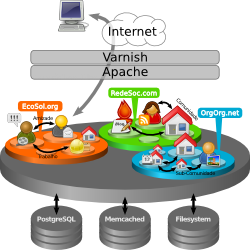
\includegraphics[scale=0.6]{estrutura-noosfero.png}
\caption{Estrutura do Noosfero}
\label{fig:estrutura-noosfero}
\end{figure}

O Noosfero é um software livre licenciado sob a  GNU Affero General
Public License\footnote{http://www.gnu.org/licenses/agpl.html} versão 3 ou superior.

\subsection{Linguagem Ruby}

\epigraph{\textit{I wanted to minimize my frustration during programming, so I
want to minimize my effort in programming. That was my primary goal in
designing Ruby. I want to have fun in programming myself.}}{Yukihiro
Matsumoto}

A linguagem de programação Ruby foi inicialmente planejada e
desenvolvida no Japão em 1993 por Yukihiro
Matsumoto, inspirado pelas
linguagens Python, Perl, Smalltalk, Ada e
Lisp\footnote{https://www.ruby-lang.org/en/about/}.

Ruby é uma linguagem orientada a objetos e não possui tipos primitivos
como em outras linguagens. Ou seja, todos os tipos de dados são objetos,
como os tipos que representam os "inteiros", "strings" e "hash". É uma
linguagem interpretada, que não precisa de compilação e executada
diretamente pelo sistema
operacional\footnote{http://pt.wikipedia.org/wiki/Linguagem\_interpretada}.
Por ser multiplataforma, pode ser executado a partir de qualquer sistema
operacional.

Possui tipagem
dinâmica\footnote{http://pt.wikipedia.org/wiki/Tipagem\_dinâmica} e
forte, então todas as variáveis pertencem a um tipo de dados mesmos sem
ter sido declarado previamente e o tipo da variável pode ser alterado
dinamicamente.

Mais informações sobre a linguagem podem ser encontradas nos sites
RubyLearning.com\footnote{http://rubylearning.com/},
The-Little-Book-Of-Ruby\footnote{http://www.sapphiresteel.com},
Tutoriais web da Colivre\footnote{https://www.colivre.coop.br/Tech} e a
API do Ruby\footnote{http://www.ruby-doc.org/core/}

\subsection{Framework Rails}

Rails é um framework livre escrito na linguagem Ruby e também é chamado
de Ruby on Rails, ou RoR. Framework é um
conjunto de classes implementadas em uma linguagem de programação
específica, usadas para auxiliar o desenvolvimento de
software\footnote{http://pt.wikipedia.org/wiki/Framework}.
Desenvolvido por David Heinemeier Hansson para facilitar a vida do
desenvolvedor e para uma {\it Web sem burocracia}. Foi lançado para o
público em 2004 e é considerado o responsável pala fama do Ruby.

É formado pelos frameworks {\it ActiveRecord}, {\it ActionPack},
{\it ActionMailer} e {\it ActiveSupport}.

Para facilitar a vida dos desenvolvedores, Rails segue dois
conceitos\footnote{http://pt.wikipedia.org/wiki/Ruby\_on\_Rails}:

\begin{itemize}
  \item \textbf{DRY} (Don't Repeat Yourself - Não se repita): é o
conceito por trás da técnica de definir nomes, propriedades e códigos em
somente um lugar e reaproveitar essas informações em outros.
  \item \textbf{Convention over configuration} (Convenção sobre
configuração): o Rails assume valores padrão onde existe uma convenção.
Mesmo assim, os valores podem ser sobrescritos na aplicação se o
desenvolvedor preferir.
\end{itemize}

Mais informações sobre o framework podem ser encontradas nos sites
Rails Guides\footnote{http://guides.rubyonrails.org},
Tutoriais web da Colivre\footnote{https://www.colivre.coop.br/Tech} e a
API do Rails\footnote{http://api.rubyonrails.org}. Muitas informações
interessantes também podem ser obtidas no livro {\it Agile Web Development
with Rails}.

\subsubsection{Arquitetura MVC}

É um modelo de arquitetura de software que foi descrito por Trygve
Reenskaug em 1979 que propõe que a aplicação seja dividida em três
tipos de componentes. A relação entre os componentes está representada
na Figura~\ref{fig:estrutura-mvc}\footnote{Fonte:
https://upload.wikimedia.org/wikipedia/commons/b/b5/ModelViewControllerDiagram2.svg}.

\begin{figure}[h]
\center
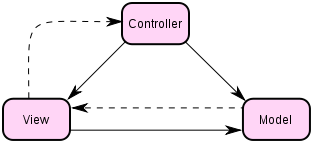
\includegraphics[scale=0.6]{mvc.png}
\caption{Estrutura do MVC}
\label{fig:estrutura-mvc}
\end{figure}

Essa arquitetura propõe a separação entre o acesso aos dados e lógica de
negócio, a lógica de apresentação e a interação com o usuário. Essa
separação facilita a reusabilidade de código e separação de conceitos.

\subsection{Varnish}

Varnish é um proxy HTTP reverso que armazena o conteúdo HTTP requisitado
no servidor, evitando que o servidor precise consultar e processar o
mesmo conteúdo diversas
vezes\footnote{https://www.varnish-cache.org/about}.

Em uma instalação padrão o Varnish não é configurado, mas é aconselhado
que os servidores utilizados em modo de produção configurem e utilizem o
Varnish por causa da melhoria de performance obtida com sua utilzação.

\subsection{Memcached}

Memcached é um sistema de cache em memória utilizado para melhorar
a performance dos sites dinâmicos, cacheando objetos na memória do
servidor, diminuindo a quantidade de acessos ao banco de
dados\footnote{http://memcached.org/}.

\subsection{PostgreSQL}

PostgreSQL é um sistema de gerenciamento de banco de dados relacional de
objetos desenvolvido como software
livre\footnote{http://www.postgresql.org/about/}.

O Noosfero é homologado para uso com o banco de dados PostgreSQL.

\subsection{Licenças de software}

Licenças de software são instrumentos legais que regulamentam o uso e
redistribuição de software. Sem considerar as particularidades de cada
licença, as licenças de um software o definem como software livre,
software de códgo aberto ou software proprietário.
Para cada definição de software, podem ser utilizadas diversas licenças.
Cada licença possui regras para uso e distribuição do software que
impactarão no software.

Órgãos como a Free Software Foundation
(FSF)\footnote{http://www.fsf.org/} e a Open Source
Initiative (OSI)\footnote{http://www.opensource.org/} apoiam e
promovem o uso e distribuição de softwares livres, fornecendo listas de
licenças para softwares livres e de código aberto.

\subsubsection{GNU Affero General Public License}

A licença utilizada no Noosfero é a licença GNU
Affero\footnote{http://www.gnu.org/licenses/agpl.html} (GNU AGPL).

Essa licença garante que os usuários do software possuem as quatro
liberdades essenciais:

\begin{itemize}
  \item A liberdade de executar o programa, para qualquer propósito (liberdade 0).
  \item A liberdade de estudar como o programa funciona, e adaptá-lo às
suas necessidades (liberdade 1). Para tanto, acesso ao código-fonte é um
pré-requisito.
  \item A liberdade de redistribuir cópias de modo que você possa ajudar
ao próximo (liberdade 2).
  \item A liberdade de distribuir cópias de suas versões modificadas a
outros (liberdade 3). Desta forma, você pode dar a toda comunidade a
chance de beneficiar de suas mudanças. Para tanto, acesso ao
código-fonte é um pré-requisito. (GNU, 2013, online).
\end{itemize}

\section{Documentação de Instalação e Utilização do Noosfero}

Essa seção documenta os passos necessários para a instalação do
Noosfero em um servidor com Debian Estável.

\subsection{Instalação}

O Noosfero é disponibilizado num repositório público para download e
instalação fácil em servidores com Debian na versão estável.

\subsubsection{Obter o pacote Debian}

O pacote para instalação em servidores Debian está disponível em um
repositório público. Para obter o pacote, o usuário
deve seguir as instruções abaixo:

\begin{enumerate}
  \item Inclusão do repositório do Noosfero no arquivo que lista as fontes de onde
os pacotes serão obtidos (/etc/apt/source.list):
    \begin{verbatim}
      deb http://download.noosfero.org/debian/squeeze ./
    \end{verbatim}
  \item Atualização da lista de pacotes:
    \begin{verbatim}
      $ sudo apt-get update
    \end{verbatim}
  \item Instalação do Noosfero
    \begin{verbatim}
      $ sudo apt-get install noosfero noosfero-apache
    \end{verbatim}
\end{enumerate}

\subsubsection{Configuração do pacote Debian}

Após o download, o usuário precisará fazer a configuração do
pacote do Noosfero:

\begin{figure}[h]
\center
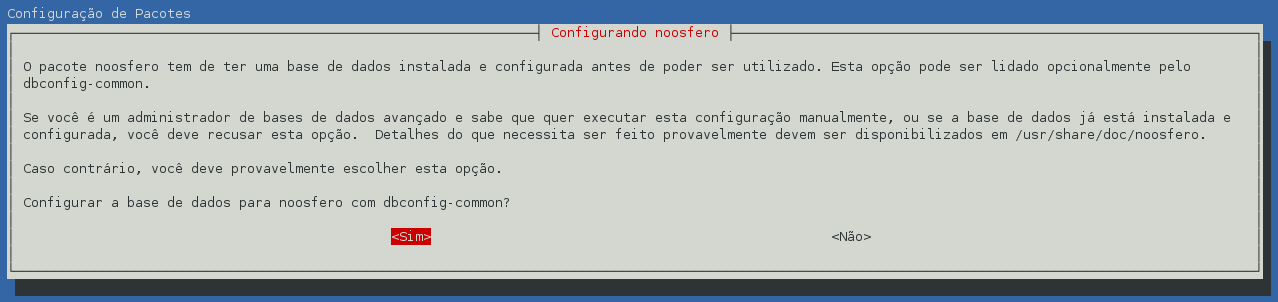
\includegraphics[scale=0.3]{1-db-common.png}
\caption{Configuração do banco de dados}
\label{fig:noosfero-db-common}
\end{figure}

\begin{figure}[h]
\center
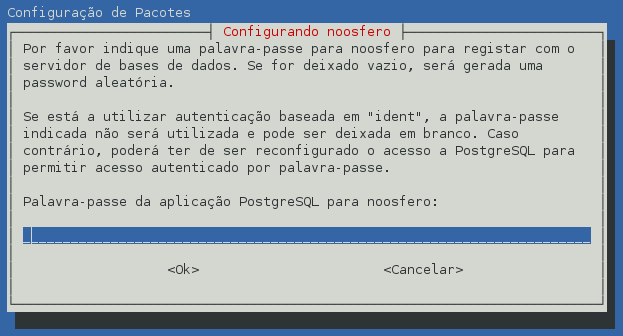
\includegraphics[scale=0.4]{password-2.png}
\caption{Senha do banco de dados}
\label{fig:noosfero-password}
\end{figure}

\begin{figure}[h]
\center
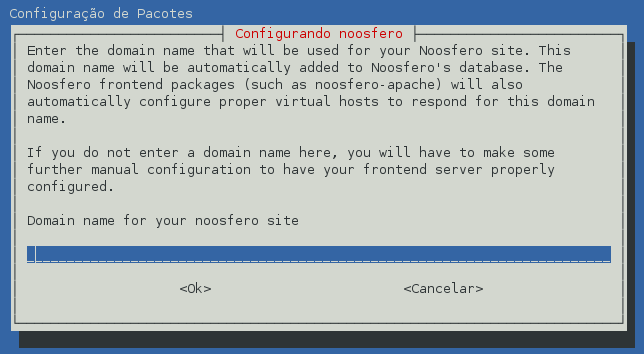
\includegraphics[scale=0.4]{domain-3.png}
\caption{Domínio da aplicação}
\label{fig:noosfero-domain}
\end{figure}

\begin{figure}[h]
\center
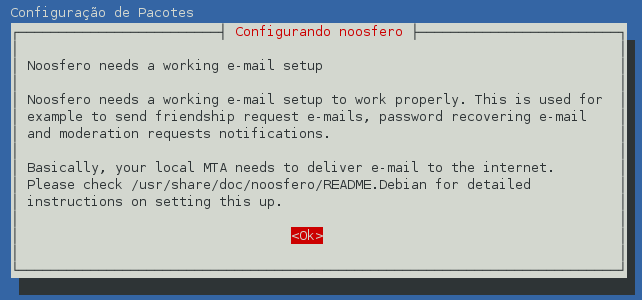
\includegraphics[scale=0.4]{email-setup-4.png}
\caption{Mensagem sobre configuração de e-mail}
\label{fig:noosfero-email-setup}
\end{figure}

\begin{enumerate}
  \item Configuração do banco de dados
(Figura~\ref{fig:noosfero-db-common}): Por padrão (Sim), o Noosfero configura
automaticamente o banco de dados para uso na aplicação. Caso o usuário
seja um administrador de banco de dados e tenha necessidade de fazer uma
configuração personalizada, deve recusar (Não) a opção e fazer as
configurações manualmente.
  \item Definição da senha do banco de dados
(Figura~\ref{fig:noosfero-password}): Essa senha será utilizado pelo
Noosfero para acessar o bando de dados.
  \item Definição do domínio
(Figura~\ref{fig:noosfero-domain}): Esse será o endereço utilizado para
acessar a instância do Noosfero. O domínio já deverá estar definido para
apontar para o endereço IP do servidor.
  \item Mensagem sobre configuração de e-mail
(Figura~\ref{fig:noosfero-email-setup}): Após a instalação do pacote a
configuração básica de envio de e-mail estará funcionando. Para outras
configurações, a documentação no código deve ser
verificada\footnote{https://gitorious.org/noosfero/noosfero/source/INSTALL.email}.
\end{enumerate}

\subsubsection{Configuração inicial do ambiente Noosfero}

Após a instalação e configuração do pacote, o ambiente estará disponível
para cadastro de novos usuários. Para administrar o ambiente é necessário que seja
criado pelo menos um usuário com o perfil de administrador e isso deve
ser feito pelo servidor:

\begin{enumerate}
  \item Acesso ao {\it console} do Noosfero como usuário {\it root} do
servidor:
    \begin{verbatim}
      # noosfero-console
    \end{verbatim}
  \item No {\it console} do Noosfero, será necessário executar o comando a seguir para
criar o usuário. Importante lembrar que
as informações devem ser substituídas com as informação do usuário
(o e-mail e senha, por exemplo, devem ser substituídos):
    \begin{verbatim}
      >> user = User.create(:login => 'adminuser',
                            :email => 'admin@example.com',
                            :password => 'admin',
                            :password_confirmation => 'admin',
                            :environment => Environment.default)
    \end{verbatim}
  \item Ainda no {\it console} do Noosfero, o usuário deverá ser
ativado:
    \begin{verbatim}
      >> user.activate
    \end{verbatim}
  \item Por fim, o usuário criado deverá ser definido como administrador
do ambiente:
    \begin{verbatim}
      >>Environment.default.add_admin user.person
    \end{verbatim}
  \item Para sair do {\it console} do Noosfero, o usuário poderá digitar
{\it exit}
\end{enumerate}

\subsection{Utilização}

A documentação de utilização do Noosfero está disponível online, na
página do Portal de Consulta
Pública\footnote{http://psocial.sg.gov.br/doc}. O manual é dividido em 7
seções e cada seção é dividida em algumas sub-seções:

\begin{itemize}
  \item Plugins
  \item Funcionalidades do empreendimento
  \item Funcionalidade de administração
  \item Funcionalidades da comunidade
  \item Navegação
  \item Gerenciamento de conteúdo
  \item Funcionalidades do usuário
\end{itemize}

Além do manual online disponível em todos as redes sociais criadas com o
Noosfero, a página oficial do Noosfero também disponibiliza alguns
vídeos\footnote{http://noosfero.org/Development/VideosPt} com
apresentações em eventos sobre como o Noosfero funciona e vídeo-aulas
feitas pela comunidade para ajudar os usuários a utilizarem a
ferramenta.

\newpage

\section{Considerações finais}

Neste documento foi apresentado o documento com complementação da 
documentação de instalação e uso da plataforma Noosfero contendo
conceitos e tutoriais.

A documentação disponível na página do
Noosfero\footnote{http://noosfero.org/Development} foi atualizada
seguindo as informações levantadas nesse documento.

\vspace{1cm}

Sem mais nada a acrescentar, coloco-me à disposição.

\vspace{1cm}

\begin{minipage}{\textwidth}
  Brasília/DF, \DiaEntrega \ de \MesEntrega\\[1cm]
  \textbf{\MyName}\\
  \small Consultora do PNUD
\end{minipage}

\end{document}
